\documentclass[journal, a4paper,11pt]{IEEEtran}

\usepackage{graphicx}

%\usepackage{subfigure} 
\usepackage{setspace}

\usepackage{url}        

%\usepackage{stfloats} 

\usepackage{amsmath}    

\usepackage{ragged2e}
\usepackage{graphicx}

\linespread{1.5}

\begin{document}

\begin{titlepage}
	\centering
    \vspace{2cm}
    {\scshape\LARGE\bfseries Physics Studies for a Very High \par Energy Electron-Proton Collider\par}
    \vspace{2cm}
	{\scshape\Large\bfseries Literature Review\par}
	\vspace{2cm}
	{\scshape\Large Department of Physics and Astrophysics\par University College London\par}
	\vspace{4cm}
	{\huge\bfseries\par}
	{\large Pranav Rao\par}
	{\large First Supervisor : Prof. Matthew Wing\par Second Supervisor: Dr. Alessio Serafini\par}
	\vspace{8cm}
	Word Count: 

	\vfill
\end{titlepage}

    
\justify
\section{Background}

\subsection*{\textbf{Deep Inelastic Scattering}}

Electron-proton collisions at sufficiently high energies result in the proton breaking up into hadrons, this process is referred to as Deep Inelastic Scattering (DIS) shown in Fig.\ref{fig:DIS}. This theory has led to the discovery that protons are composite particles containing three valance quarks. While elastic scattering, where the proton is not broken up, do occur at high energies as well, DIS is the dominant collision type at high energies.

\begin{figure}[!h]
	\centering
		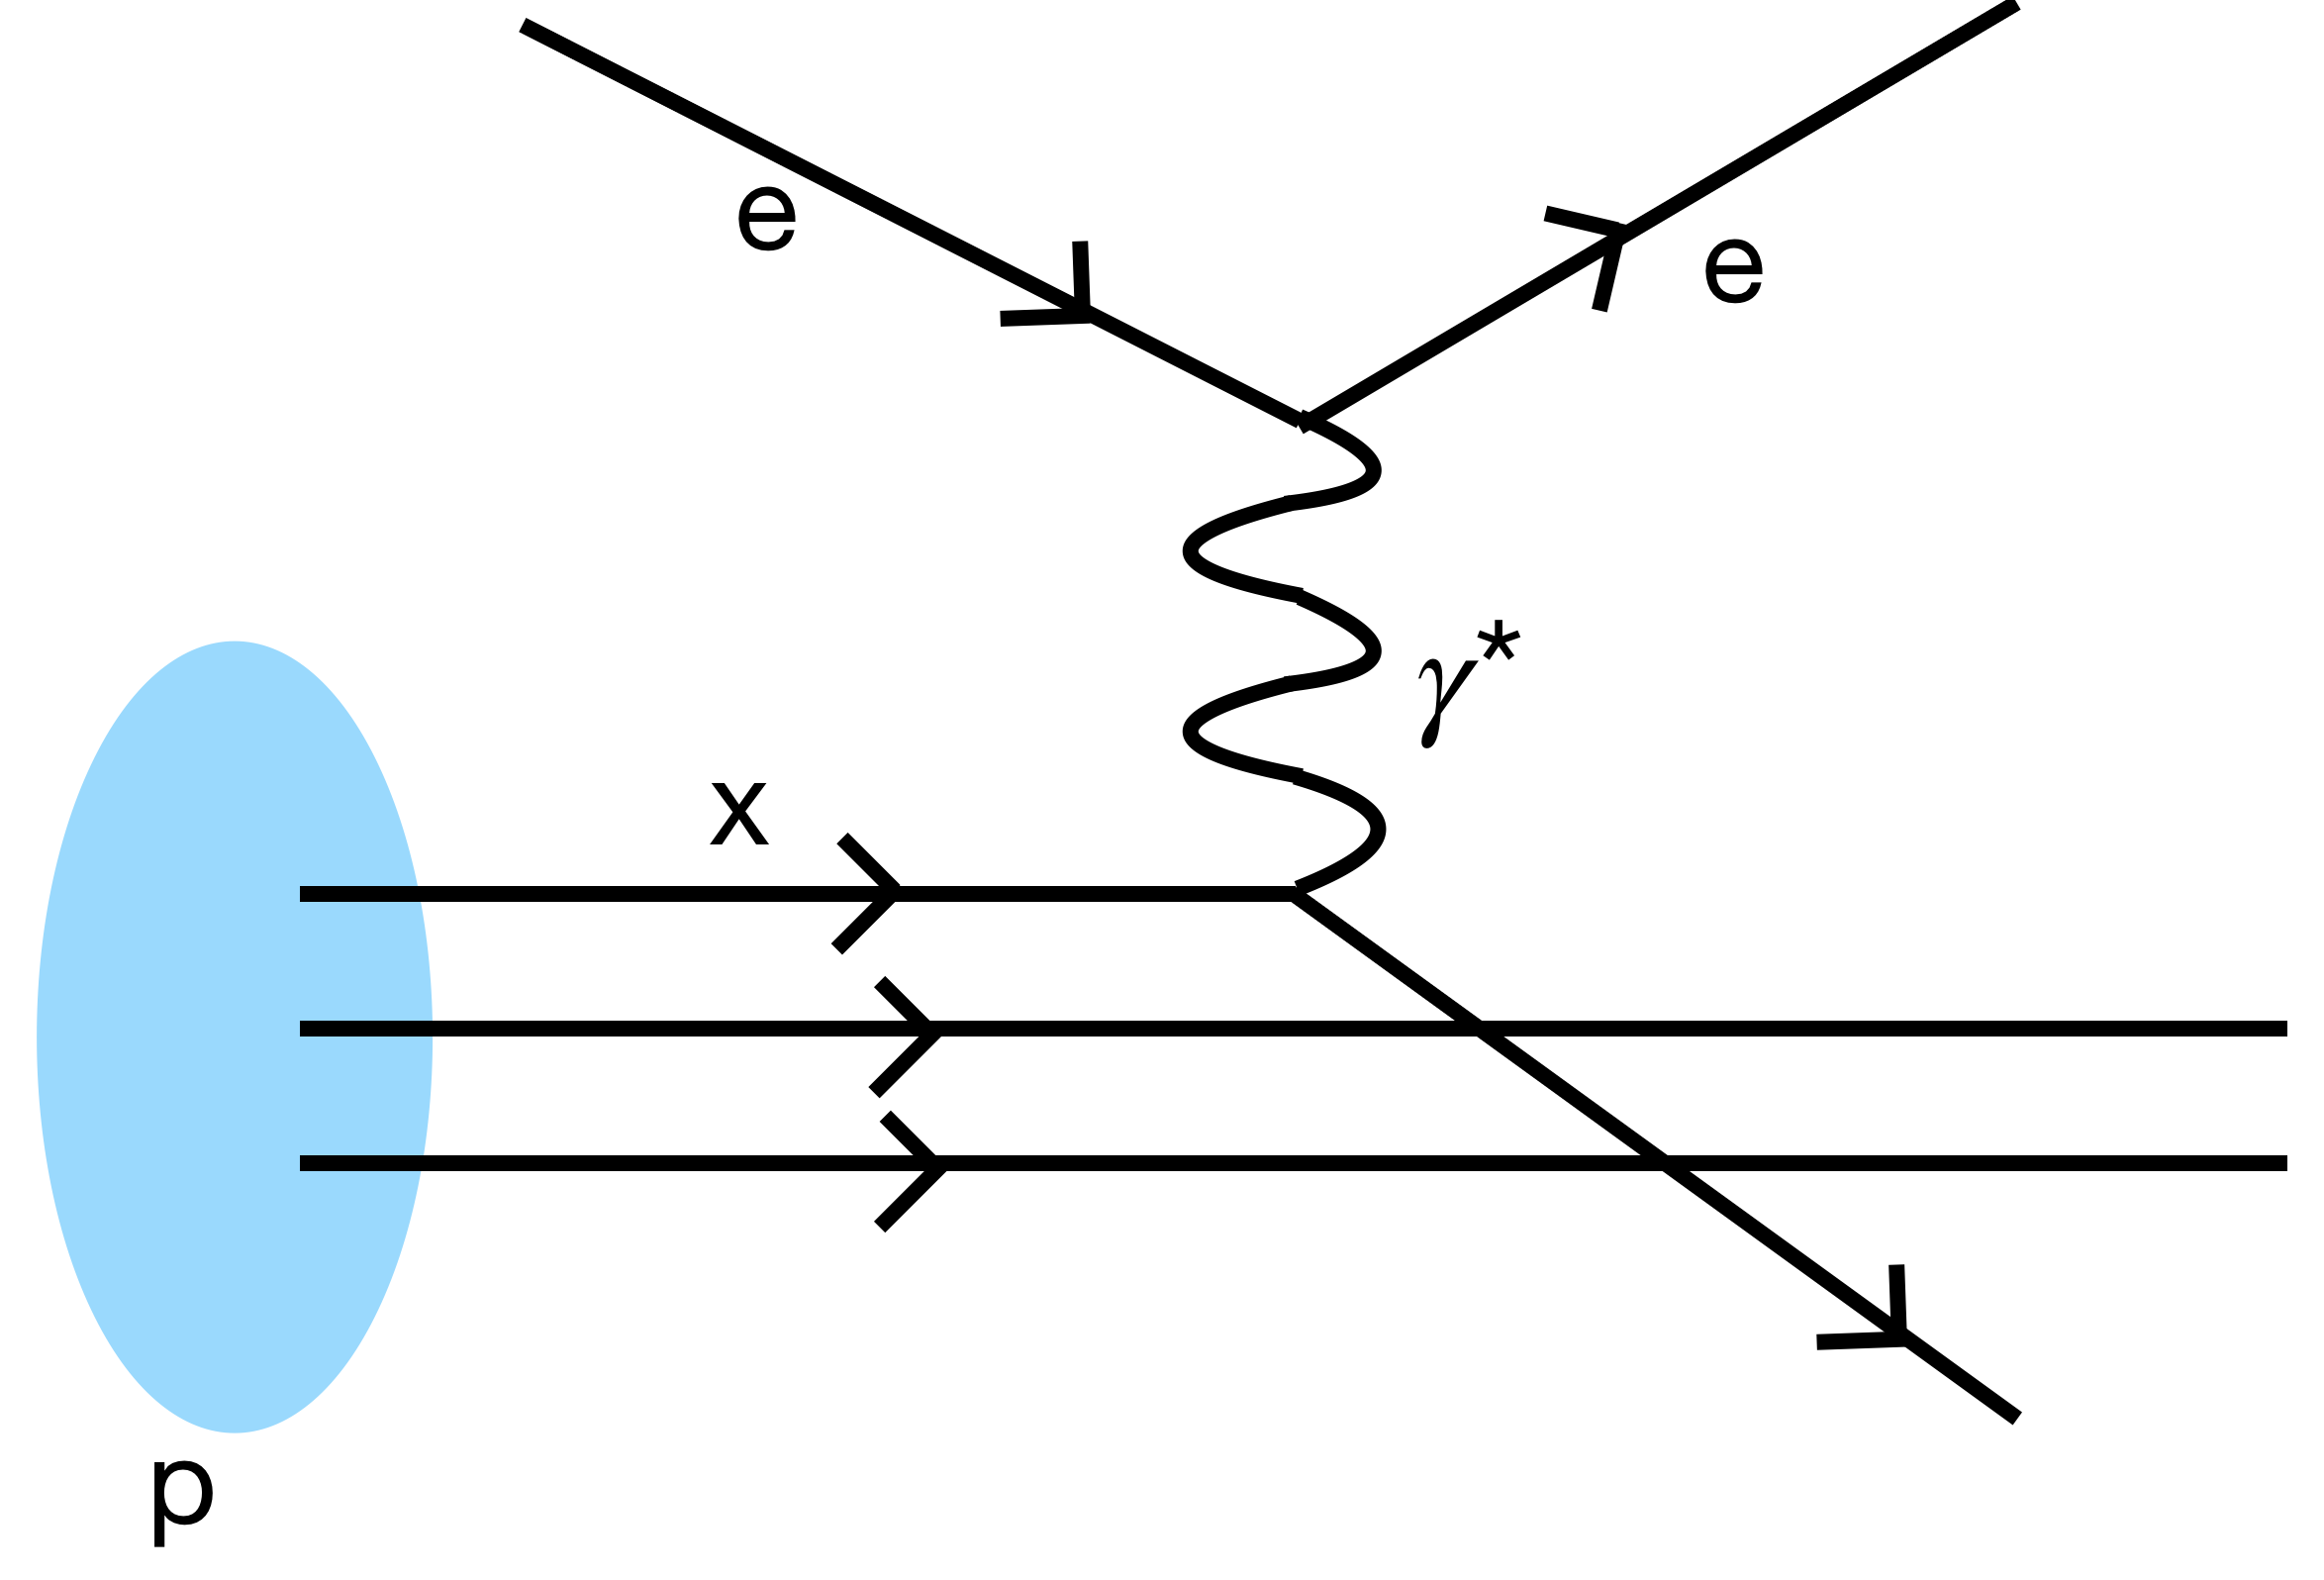
\includegraphics[width =0.4\textwidth]{DIS.png}
		\caption{Schematic diagram showing deep inelastic scattering.}
		\label{fig:DIS}
\end{figure}

The hadronic final state consists of many particles and as a result its invariant mass can have a range of values unlike elastic scattering where the invariant mass of the final state is the mass of the proton. This range of values leads to an additional degree of freedom which requires an additional quantity to describe the kinematics of the event. The quantities required are chosen from a list of Lorentz invariant quantities x, y, $\nu$, and $Q^2$. 
The energies at which DIS occurs are high enough to neglect the mass of the electrons while making predictions, as a result a good approximation of $Q^2$ can be made \cite{Modern}:
\begin{equation}
	Q^2 = 4E_1E_3sin^2\frac{\theta}{2}
	\label{eq:Q2}
\end{equation}
which is always positive. In eq \ref{eq:Q2} $Q^2$ is the four-momentum squared, $E_1$ is the energy of the
%Bjorken x
Bjorken $x$ is one of the Lorentz invariant quantities that can be used to describe kinematics of DIS. It is given by the following equation \cite{Modern}: 
\begin{equation}
	x = \frac{Q^2}{Q^2 + W^2 - m_p^2}
	\label{eq:x}
\end{equation}
where $Q^2$ is the four-momentum transferred, $W^2$ is the invariant mass of the hadronic state, and $m_p^2$ is the rest mass of the proton squared. $W^2 \geq m_p^2$ because for baryon number to be conserved, the hadronic state must contain one baryon and the proton is the lightest baryon. $W^2 - m_p^2 \geq 0$ along with $Q^2 \geq 0$ gives the range $0 \leq x \leq 1$. Bjorken $x$ is a variable that describes the elasticity of the scattering process, and when $x = 1$ the scattering process is elastic and $Q^2 = W^2$.

Another Lorentz invariant dimensionless quantity used to describe DIS kinetics is the inelasticity $y$ and it is defined as follows \cite{Modern}:
\begin{equation}
	y = 1-\frac{E_3}{E_1}.
	\label{eq:y}
\end{equation}
The inelasticity can also be understood as the fractional loss in electron energy which also has a range $0 \leq y \leq 1$.

In situations where it is more convenient to work with the energy difference rather than the fractional energy lost the Lorentz invariant quantity $\nu$ is used, and it is described as \cite{Modern}:
\begin{equation}
	\nu = E_1 - E_3,
	\label{eq:nu}
\end{equation}
and can be understood as the absolute energy lost by the electron in the scattering process.
The kinematics of a DIS collision can be described using any combination of $Q^2$, $x$, $y$, and $\nu$ for a fixed centre of mass energy, except for $y$ and $\nu$ because they are not independent of each-other.

\subsection*{\textbf{Plasma Wakefield Acceleration}}

Plasma wakefield acceleration is a technique used for linearly accelerating electrons to sufficiently high energies which have not been achieved before. The biggest advantage this has over radio frequency (RF) acceleration is its ability to reach very high electric fields, which allows the set up to be extremely compact \cite{0409}. 

The new frontier of colliders are thought to be electron-positron colliders with very high centre of mass energies, however the main challenge to over come is being unable to accelerate electrons above 100 MeV using RF technology \cite{0114}. To excite electrons to TeV scale linear accelerators would need to be tens of Kms long and circular accelerators would need to be hundreds of Kms long with the technology available today \cite{0114}. Electrons can be accelerated to TeV scales using a wakefield within tens of metres \cite{0409}, as a result plasma wakefield acceleration could be critical for the development of next generation particle colliders.

Plasmas are capable of sustaining $10 GeV/m$ potential gradients which is several orders of magnitudes greater than what RF accelerators are capable of achieving. Plasmas support near light speed waves or wakes which is the key mechanism for accelerating electrons. These wakes are made of longitudinal and transverse components, the longitudinal component provides the electrons with the acceleration and the transverse components focuses the electron bunch. The transverse component has a focusing power many orders larger than conventional magnets used for focusing \cite{0114}.

Proton driven plasma wakefield acceleration is the next step for particle colliders to advance, however there is a challenge that needs to be overcome: the current length of of proton bunches used to drive the wakefield is too long. Plasmas have an oscillating frequency which needs to be met by the driving frequency to achieve resonance. Plasmas which can provide GeV/m potential have a wavelength in the mm scale, while proton bunches are much longer, in the cm scale \cite{0114}.

One solution is self modulating instability (SMI), this is a mechanism by which the driving frequency can be made to match the plasma frequency. SMI splits bunches of protons into micro bunches which reduces the wavelength of the driving proton beam. Under the right conditions the wavelength can be made to exactly equal exactly one plasma wavelength, achieving resonance. Despite SMI being energy inefficient, it is cost effective and relatively simple to execute, as a result it is a good starting point to use in the proof of concept for wakefield acceleration \cite{1115}.

\section{HERA Collider and H1 Collaboration}

HERA was a electron-proton collider that ran from 1997-2007 and had a circumference of 6.3 Km. Electrons were accelerated to $\approx 27.5$ GeV and collided with protons that were accelerated to $\approx 900$ GeV \cite{Modern}. It operated with a centre of mass energy of $\sqrt{s} = 318 GeV$, which was the highest centre of mass for a $ep$ collider \cite{1308}.

The H1 collaboration \cite{H1} was one of the experiments that was located at HERA. Ref \cite{H1} presents measurements of jet cross sections in neutral current (NC) DIS for $5.5 \leq Q^2 \leq 80 GeV^2$ with inelasticities $0.2 \leq y \leq 0.6$. 

If quarks were composite particles then deviations from the Bjorken scaling would be expected when the wavelength of the virtual photon was comparable to the size of the quark. As the data colleced by H1 was consistent with Bjorken scalling, the radius of the quark was predicted to be smaller than $10^{-18}m$.

\subsection*{\txtbf{Rivet Analysis of H1 Collaboration}}

Robust Independent Validation of Experiment and Theory (Rivet) is a toolkit which is used as a method of validating theory with the use of Monte Carlo (MC) event generators. It has a host of various analyses, with the capability of writing your own. 

One of the main aims is to write a complete Rivet analysis for the H1 paper \cite{H1}. By writing a Rivet routine it would be possible run theory cross checks and extrapolate, to some extent, the theory for very high energies. This extrapolation could provide a comparison to the experimental data of very high energy DIS collisions, and is a good starting point for testing the differences between DIS at low and high energy frames.


\section{Timeline}



\bibliographystyle{ieeetr}
\bibliography{bib.bib}



\end{document}






